\chapter{FieldMap Toolbox \label{Chap:FieldMap}}

\section{Introduction}

This chapter describes how to use the FieldMap toolbox version 2.1\footnote{
FieldMap Version 2.0 can be downloaded as part of SPM:
\url{http://www.fil.ion.ucl.ac.uk/spm/software/}\\
FieldMap Version 1.1 for SPM2 can be downloaded from
\url{http://www.fil.ion.ucl.ac.uk/spm/toolbox/fieldmap/}}
 for creating unwrapped field maps that can be used to do geometric distortion correction of EPI images \cite{chloe_distortion,chloe_distortion2,ja_geometric}. The methods are based on earlier work by Jezzard et al.,\cite{jezzard95} and a phase-unwrapping algorithm by Jenkinson \cite{jenkinson03}. The toolbox can be used via the SPM batch editor or in an interactive mode so that the user can see the effect of applying different field maps and unwarping parameters to EPI images. A voxel displacement map (VDM) is created that can be used with Realign \& Unwarp for doing a combined static and dynamic distortion correction or with an Apply VDM function for doing a static distortion correction on a set of realigned images. Realign \& Unwarp is designed to work only with images acquired with the phase-encode direction aligned with the anterior-posterior axis. Images acquired with phase-encode directions aligned with other axes can be distortion corrected using the FieldMap toolbox and Apply VDM utility.

\begin{figure}
\begin{center}
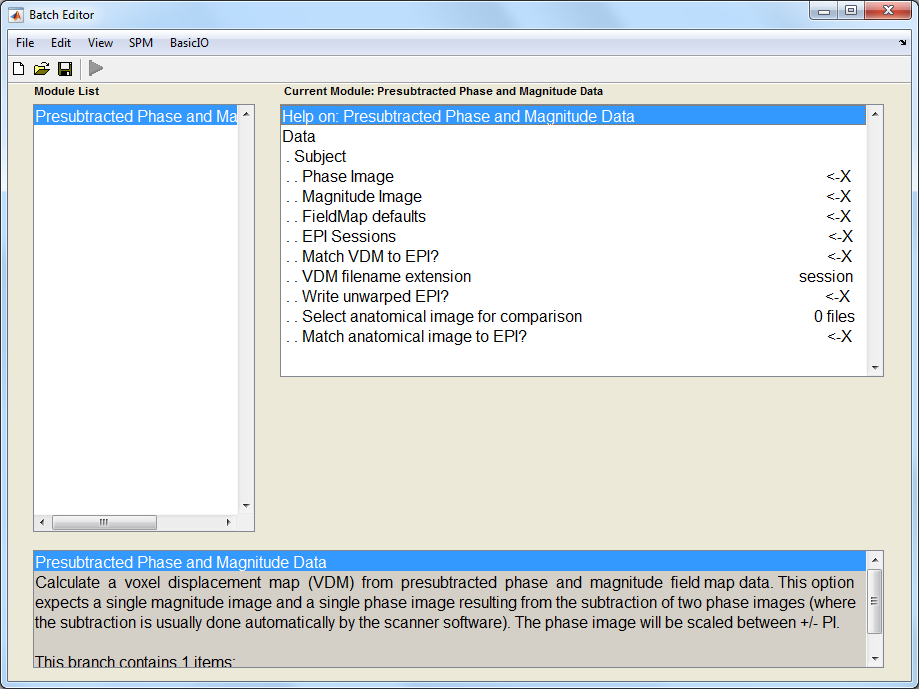
\includegraphics[width=100mm]{FieldMap/fieldmap_taskmgr}
\end{center}
\caption{FieldMap using the SPM User Interface.\label{FM1}}
\end{figure}

\section{Presubtracted Phase and Magnitude Data}
Calculate a voxel displacement map (VDM) from presubtracted phase and magnitude field map data (Figure \ref{FM1}). This option expects a single magnitude image and a single phase image resulting from the subtraction of two phase images (where the subtraction is usually done automatically by the scanner software). The phase image will be scaled between +/- PI.


\subsection{Data}
Subjects or sessions for which individual field map data has been acquired.


\subsubsection{Subject}
Data for this subject or field map session.


\paragraph{Phase Image}
Select a single phase image. This should be the result from the subtraction of two phase images (where the subtraction is usually done automatically by the scanner software). The phase image will be scaled between +/- PI.


\paragraph{Magnitude Image}
Select a single magnitude image. This is used for masking the phase information and coregistration with the EPI data. If two magnitude images are available, select the one acquired at the shorter echo time because it will have greater signal


\paragraph{FieldMap defaults}
FieldMap default values can be entered as a file or set of values.


\subparagraph{Defaults values}
Defaults values


\textbf{Echo times [short TE long TE]}
Enter the short and long echo times (in ms) of the data used to acquire the field map.


\textbf{Mask brain}
Select masking or no masking of the brain. If masking is selected, the magnitude image is used to generate a mask of the brain.


\textbf{Blip direction}
Enter the blip direction. This is the polarity of the phase-encode blips describing the direction in which k-space is traversed along the y-axis during EPI acquisition with respect to the coordinate system used in SPM. In this coordinate system, the phase encode direction corresponds with the y-direction and is defined as positive from the posterior to the anterior of the head.

The convention used to describe the direction of the k-space traversal is based on the coordinate system used by SPM. In this coordinate system, the phase encode direction corresponds with the y-direction and is defined as positive from the posterior to the anterior of the head. The x-direction is defined as positive from left to right and the z-direction is defined as positive from foot to head. The polarity of the phase-encode blips describes in which direction k-space is traversed along the y-axis with respect to the coordinate system described here. 

\textbf{Total EPI readout time}
Enter the total EPI readout time (in ms). This is the time taken to acquire all of the phase encode steps required to cover k-space (ie one image slice). For example, if the EPI sequence has 64 phase encode steps, the total readout time is the time taken to acquire 64 echoes, e.g. total readout time = number of echos x echo spacing. This time does not include i) the duration of the excitation, ii) the delay between, the excitation and the start of the acquisition or iii) time for fat saturation etc.


\textbf{EPI-based field map?}
Select non-EPI or EPI based field map. The field map data may be acquired using a non-EPI sequence (typically a gradient echo sequence) or an EPI sequence. The processing will be slightly different for the two cases. If using an EPI-based field map, the resulting Voxel Displacement Map will be inverted since the field map was acquired in distorted space.


\textbf{Jacobian modulation?}
Select whether or not to use Jacobian modulation. This will adjust the intensities of voxels that have been stretched or compressed but in general is not recommended for EPI distortion correction


\textbf{uflags}
Different options for phase unwrapping and field map processing


\textsc{Unwrapping method}
Select method for phase unwrapping


\textsc{FWHM}
FWHM of Gaussian filter used to implement weighted smoothing of unwrapped maps.


\textsc{pad}
Size of padding kernel if required.


\textsc{Weighted smoothing}
Select normal or weighted smoothing.


\textbf{mflags}
Different options used for the segmentation and creation of the brain mask.


\textsc{Template image for brain masking}
Select template file for segmentation to create brain mask


\textsc{FWHM}
FWHM of Gaussian filter for smoothing brain mask.


\textsc{Number of erosions}
Number of erosions used to create brain mask.


\textsc{Number of dilations}
Number of dilations used to create brain mask.


\textsc{Threshold}
Threshold used to create brain mask from segmented data.


\textsc{Regularization}
Regularization value used in the segmentation. A larger value helps the segmentation to converge.


\subparagraph{Defaults File \label{PMDEF}}
Select the 'pm\_defaults*.m' file containing the parameters for the field map data. Please make sure that the parameters defined in the defaults file are correct for your field map and EPI sequence. To create your own customised defaults file, either edit the distributed version and/or save it with the name 'pm\_defaults\_yourname.m'.


\paragraph{EPI Sessions}
If a single set of field map data will be used for multiple EPI runs/sessions, select the first EPI in each run/session. A VDM file will created for each run/session, matched to the first EPI in each run/session and saved with a unique name extension.


\subparagraph{Session}
Data for this session.


\textbf{Select EPI to Unwarp}
Select a single image to distortion correct. The corrected image will be saved with the prefix u. Note that this option is mainly for quality control of correction so that the original and distortion corrected images can be displayed for comparison. To unwarp multiple images please use either Realign \& Unwarp or Apply VDM.


\paragraph{Match VDM to EPI?}
Match VDM file to EPI image. This will coregister the field map data to the selected EPI for each run/session.

In general, the field map data should be acquired so that it is as closely registered with the EPI data as possible but matching can be selected if required. If a precalculated field map was loaded then the user is prompted to select a magnitude image in the same space as the field map. If real and imaginary images were selected, the toolbox automatically creates a magnitude image from these images and saves it with the name mag\_NAME-OF-FIRST-INPUT-IMAGE.img. 

\paragraph{Name extension for run/session specific VDM file}
This will be the name extension followed by an incremented integer for run/session specific VDM files.


\paragraph{Write unwarped EPI?}
Write out distortion corrected EPI image. The image is saved with the prefix u. Note that this option is mainly for quality control of correction so that the original and distortion corrected images can be displayed for comparison. To unwarp multiple images please use either Realign \& Unwarp or Apply VDM.


\paragraph{Select anatomical image for comparison}
Select an anatomical image for comparison with the distortion corrected EPI or leave empty. Note that this option is mainly for quality control of correction.


\paragraph{Match anatomical image to EPI?}
Match the anatomical image to the distortion corrected EPI. Note that this option is mainly for quality control of correction allowing for visual inspection and comparison of the distortion corrected EPI.


\section{Real and Imaginary Data}
Calculate a voxel displacement map (VDM) from real and imaginary field map data. This option expects two real and imaginary pairs of data of two different echo times. The phase images will be scaled between +/- PI.


\subsection{Data}
Subjects or sessions for which individual field map data has been acquired.


\subsubsection{Subject}
Data for this subject or field map session.


\paragraph{Short Echo Real Image}
Select short echo real image


\paragraph{Short Echo Imaginary Image}
Select short echo imaginary image


\paragraph{Long Echo Real Image}
Select long echo real image


\paragraph{Long Echo Imaginary Image}
Select long echo imaginary image

\paragraph{Other inputs}
As for Presubtracted Phase and Magnitude Data.

\section{Phase and Magnitude Data}
Calculate a voxel displacement map (VDM) from double phase and magnitude field map data. This option expects two phase and magnitude pairs of data of two different echo times.


\subsection{Data}
Subjects or sessions for which individual field map data has been acquired.


\subsubsection{Subject}
Data for this subject or field map session.


\paragraph{Short Echo Phase Image}
Select short echo phase image


\paragraph{Short Echo Magnitude Image}
Select short echo magnitude image


\paragraph{Long Echo Phase Image}
Select long echo phase image


\paragraph{Long Echo Magnitude Image}
Select long echo magnitude image

\paragraph{Other inputs}
As for Presubtracted Phase and Magnitude Data.

\section{Precalculated FieldMap (in Hz)}
Calculate a voxel displacement map (VDM) from a precalculated field map. This option expects a processed field map (ie phase unwrapped, masked if necessary and scaled to Hz). Precalculated field maps can be generated by the FieldMap toolbox and stored as fpm\_* files.


\subsection{Data}
Subjects or sessions for which individual field map data has been acquired.


\subsubsection{Subject}
Data for this subject or field map session.


\paragraph{Precalculated field map}
Select a precalculated field map. This should be a processed field map (ie phase unwrapped, masked if necessary and scaled to Hz) , for example as generated by the FieldMap toolbox and are stored with fpm\_* prefix.


\paragraph{Select magnitude image in same space as fieldmap}
Select magnitude image which is in the same space as the field map to do matching to EPI.

\paragraph{Other inputs}
As for Presubtracted Phase and Magnitude Data.

\section{Apply VDM }
Apply VDM (voxel displacement map) to resample voxel values in selected image(s). This allows a VDM to be applied to any images which are assumed to be already realigned (e.g. including EPI fMRI time series and DTI data).

The VDM can be been created from a field map acquisition using the FieldMap toolbox and comprises voxel shift values which describe geometric distortions occuring as a result of magnetic susceptbility artefacts. Distortions along any single dimension can be corrected therefore input data may have been acquired with phase encode directions in X, Y (most typical) and Z.

The selected images are assumed to be realigned to the first in the time series (e.g. using Realign: Estimate) but do not need to be resliced. The VDM is assumed to be in alignment with the images selected for resampling (note this can be achieved via the FieldMap toolbox). The resampled images are written to the input subdirectory with the same (prefixed) filename.

e.g. The typical processing steps for fMRI time series would be 1) Realign: Estimate, 2) FieldMap to create VDM, 3) Apply VDM.

Note that this routine is a general alternative to using the VDM in combination with Realign \& Unwarp which estimates and corrects for the combined effects of static and movement-related susceptibility induced distortions. Apply VDM can be used when dynamic distortions are not (well) modelled by Realign \& Unwarp (e.g. for fMRI data acquired with R-$>$L phase-encoding direction, high field fMRI data or DTI data).


\subsection{Data}
Subjects or sessions for which VDM file is being applied to images.


\subsubsection{Session}
Data for this session.


\paragraph{Images}
Select scans for this session. These are assumed to be realigned to the first in the time series (e.g. using Realign: Estimate) but do not need to be resliced


\paragraph{Fieldmap (vdm* file)}
Select VDM (voxel displacement map) for this session (e.g. created via FieldMap toolbox). This is assumed to be in alignment with the images selected for resampling (note this can be achieved via the FieldMap toolbox).


\subsection{Reslice Options}
Apply VDM reslice options


\subsubsection{Distortion direction}
In which direction are the distortions? Any single dimension can be corrected therefore input data may have been acquired with phase encode directions in Y (most typical), X or Z


\subsubsection{Reslice which images ?}
All Images (1..n) 

  This applies the VDM and reslices all the images. 

All Images + Mean Image 

   This applies the VDM reslices all the images and creates a mean of the resliced images.


\subsubsection{Interpolation}
The method by which the images are sampled when being written in a different space. Nearest Neighbour is fastest, but not recommended for image realignment. Trilinear interpolation is probably OK for PET, but not so suitable for fMRI because higher degree interpolation generally gives better results \cite{thevenaz00a,unser93a,unser93b}. Although higher degree methods provide better interpolation, but they are slower because they use more neighbouring voxels.


\subsubsection{Wrapping}
This indicates which directions in the volumes the values should wrap around in.  For example, in MRI scans, the images wrap around in the phase encode direction, so (e.g.) the subject's nose may poke into the back of the subject's head. These are typically:

    No wrapping - for PET or images that have already                   been spatially transformed. Also the recommended option if                   you are not really sure.

    Wrap in  Y  - for (un-resliced) MRI where phase encoding                   is in the Y direction (voxel space) etc.


\subsubsection{Masking}
Because of subject motion, different images are likely to have different patterns of zeros from where it was not possible to sample data. With masking enabled, the program searches through the whole time series looking for voxels which need to be sampled from outside the original images. Where this occurs, that voxel is set to zero for the whole set of images (unless the image format can represent NaN, in which case NaNs are used where possible).


\subsubsection{Filename Prefix}
Specify the string to be prepended to the filenames of the distortion corrected image file(s). Default prefix is 'u'.

\begin{figure}
\begin{center}
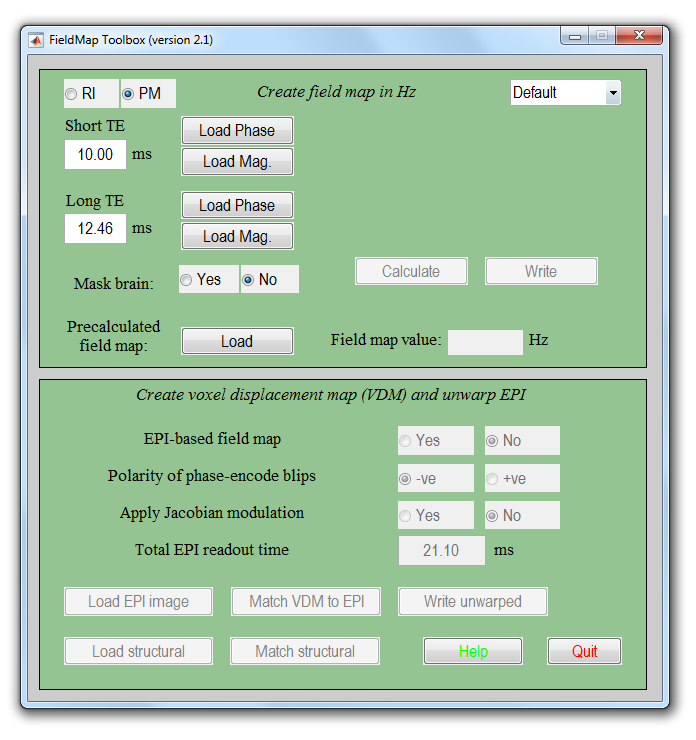
\includegraphics[width=70mm]{FieldMap/fieldmap_gui1}
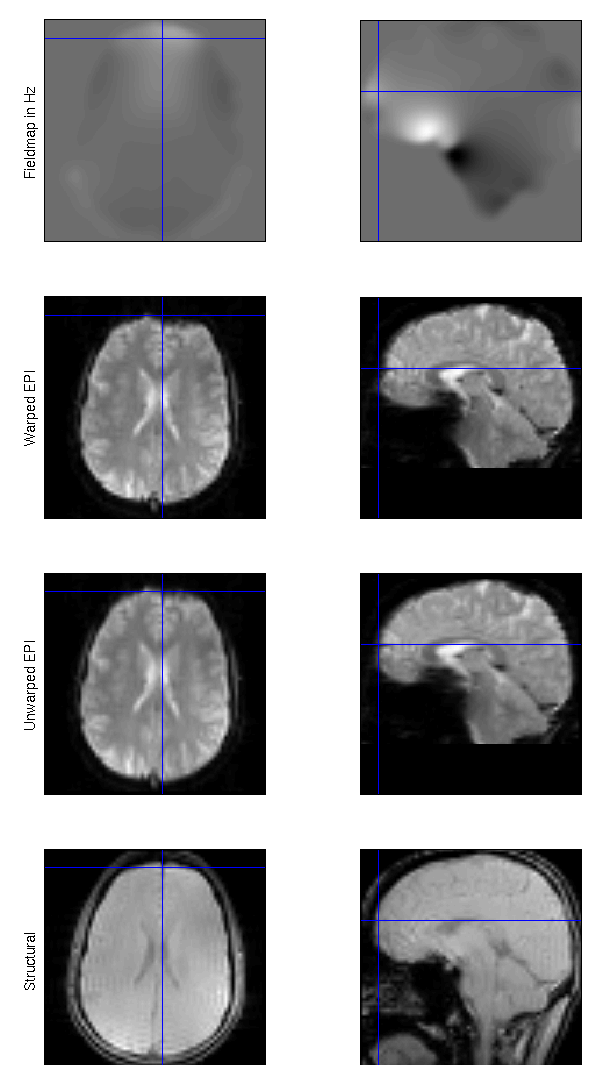
\includegraphics[width=70mm]{FieldMap/fieldmap_results1}
\end{center}
\caption{FieldMap GUI and Results. \label{FM2}}
\end{figure}

\section{Creating Field Maps Using the FieldMap GUI}
The FieldMap Toolbox GUI is shown on the left Figure \ref{FM2}. It is divided into two parts. The top part deals with creating the field map in Hz and the bottom part deals with creating the voxel displacement map (VDM) and unwarping the EPI. The toolbox can be used by working through the different inputs in the following order:

\subsection{Create field map in Hz}

\subsubsection{Load defaults file \label{loaddefs}}
Select the defaults file from which to load default parameters. If necessary, the parameters used to create the field map can be temporarily modified using the GUI. To change the default parameters, edit \texttt{pm\_defaults.m} or create a new file called \texttt{pm\_defaults\_NAME.m} (as described in Section \ref{PMDEF}).

\subsubsection{Data Input Format}
{\bf PM} The acquired field map images are in phase and magnitude format. There may be a single pair of phase and magnitude images (i.e. 2 images) in which case the phase image has been created by the vendor sequence from two echo times acquisitions. Alternatively there may be two pairs of phase and magnitude images, one for each echo time(ie 4 images). The units for the phase images MUST BE RADIANS BETWEEN +pi and -pi. The user will be asked if this is required when the images are selected.

{\bf RI} The acquired field map images are in real and imaginary format. Two pairs of real and imaginary image volumes, one for a shorter and one for a longer echo time (ie 4 images)\footnote{
NB If using SPM2, the data input format can only be changed by editing the spm\_defaults.m file. This is described in Section \ref{PMDEF}.}.

\subsubsection{File Selection}
Select NIfTI format images. Generally, the acquired scanner files will be in dicom format which can be correctly converted using the DICOM converter in the corresponding version of SPM. DICOM and other image formats can also be converted to using MRIcro\footnote{MRIcro is freely available from \url{http://www.cla.sc.edu/psyc/faculty/rorden/mricro.html}.}.

If the data input format is PM, load Phase and Magnitude images:
\begin{enumerate}
\item{Single phase image OR phase of short echo-time image.}
\item{Single magnitude image OR magnitude of short echo-time image.}
\item{LEAVE EMPTY if input consists of a single phase and magnitude pair OR phase of long echo-time image.}
\item{LEAVE EMPTY if input consists of a single phase and magnitude pair OR magnitude of long echo-time image.}
\end{enumerate}
OR 
If the data input format is RI, load Real and Magnitude images:
\begin{enumerate}
\item{Real part of short echo-time image.}
\item{Imaginary part of short echo-time image.}
\item{Real part of long echo-time image.}
\item{Imaginary part of long echo-time image.}
\end{enumerate}

\subsubsection{Short TE/Long TE (ms)}
Specify the short and long echo times in ms associated with the field map acquisition. Both of these values are required even if a single phase and magnitude image is used as input.

\subsubsection{Mask brain}
Specify yes to generate a brain mask using the magnitude data which will be used to exclude regions of the field map outside of the brain.

\subsubsection{Calculate}
Calculate an unwrapped field map in Hz which is stored in memory. This represents the map of phase changes associated with the measured field map data. The processing is described in more detail in Section \ref{FMAppendix} and involves some or all of the following steps (as specified in spm\_defaults.m): 
\begin{enumerate}
\item{Calculation of a Hz fieldmap from input data}
\item{Segmentation to exclude regions outside of the brain}
\item{Phase unwrapping}
\item{Smoothing and dilation of the processed fieldmap}
\end{enumerate}

The processed field map (in Hz) is displayed in the graphics window (top row, right Figure \ref{FM1}) and the field at different points can be explored. The field map in Hz is converted to a VDM (voxel displacement map) using the parameters shown in the FieldMap GUI and saved with the filename vdm5\_NAME-OF-FIRST-INPUT-IMAGE.img in the same directory as the acquired field map images. The VDM file is overwritten whenever the field map is recalculated or when any parameters are changed. The resulting VDM file can be used for unwarping the EPI using Realign \& Unwarp in SPM (see Section \ref{VDMuse}).

\subsubsection{Write}
Write out the processed field map (in Hz) as a Nifti format image. The image will be saved with the filename fpm\_NAME-OF-FIRST-INPUT-IMAGE.img in the same directory as the acquired field map images.

\subsubsection{Load Pre-calculated}
Load a precalculated unwrapped field map (\texttt{fpm\_\*.img}). This should be a single image volume with units of Hz in NIfTI format. The precalculated field map may have been created previously using the FieldMap toolbox or by other means. Once loaded, the field map is displayed in the graphics window (top row, right, Figure \ref{FM1}) and the field at different points can be explored.

\subsubsection{Field map value (Hz)}
Interrogate the value of the field map in Hz at the location specified by the mouse pointer in the graphics window.

\subsection{Create voxel displacement map (VDM) and unwarp EPI}

When any of the parameters below are changed, a new VDM is created and written out as vdm5\_NAME-OF-FIRST-INPUT-IMAGE.img. The vdm5\_NAME-OF-FIRST-INPUT-IMAGE.mat file is not updated unless 'Match VDM to EPI' is selected as described in Section \ref{VDMmatch}.

\subsubsection{EPI-based field map - Yes/No}
Select Yes if the field map is based on EPI data or No otherwise. Most scanner vendor field map sequences are non-EPI.

\subsubsection{Polarity of phase-encode blips - +ve/-ve}
Select +ve or -ve blip direction.When images are acquired K-space can be traversed using positive or negative phase-encode blips. This direction will influence the geometric distortions in terms of whether the affected regions of the image are stretched or compressed. 

The convention used to describe the direction of the k-space traversal is based on the coordinate system used by SPM. In this coordinate system, the phase encode direction corresponds with the y-direction and is defined as positive from the posterior to the anterior of the head. The x-direction is defined as positive from left to right and the z-direction is defined as positive from foot to head. The polarity of the phase-encode blips describes in which direction k-space is traversed along the y-axis with respect to the coordinate system described here. 

\subsubsection{Apply Jacobian modulation - Yes/No}
Select Yes to do Jacobian Modulation to adjust the intensities of voxels that have been stretched or compressed. In general this is not recommended for unwarping EPI data at this stage.

\subsubsection{Total EPI readout time (ms)}
Enter the total time in ms for the readout of the EPI echo train which is typically 10s of ms. This is the time taken to acquire all of the phase encode steps required to cover k-space (ie one image slice). For example, if the EPI sequence has 64 phase encode steps, the total readout time is the time taken to acquire 64 echoes: 
        total readout time = number of echoes $\times$ echo spacing.
This time does not include i) the duration of the excitation, ii) the delay between the excitation and the start of the acquisition or iii) time for fat saturation.

\subsubsection{Load EPI image}
Select a sample EPI image in NIfTI format. This image is automatically unwarped using the VDM calculated with the current parameters. The warped and the unwarped image are displayed in the graphics window underneath the field map (middle rows, right, Figure \ref{FM1}).

\subsubsection{Match VDM to EPI \label{VDMmatch}}
Select this option to match the field map magnitude data to the EPI image before it is used to unwarp the EPI. In general, the field map data should be acquired so that it is as closely registered with the EPI data as possible but matching can be selected if required. If a precalculated field map was loaded then the user is prompted to select a magnitude image in the same space as the field map. If real and imaginary images were selected, the toolbox automatically creates a magnitude image from these images and saves it with the name mag\_NAME-OF-FIRST-INPUT-IMAGE.img. 

\subsubsection{Write unwarped}
Write unwarped EPI image with the filename \texttt{uNAME\_OF\_EPI.img}.

\subsubsection{Load structural}
Load a structural image for comparison with unwarped EPI. This is displayed in the graphics window below the other images (bottom row, right fig 1).

\subsubsection{MatchStructural}
Coregister the structural image to the unwarped EPI and write the resulting transformation matrix to the header of the selected structural image.

\subsubsection{Help}
Call \texttt{spm\_help} to display \texttt{FieldMap.man}.

\subsubsection{Quit}
Quit the toolbox and closes all windows associated with it.


\section{Using the FieldMap in Batch scripts}
\texttt{FieldMap\_preprocess.m} which calls \texttt{FieldMap\_create.m} gives an example of how to run the FieldMap toolbox without using the GUI. To run the script, make sure your \matlab\ path includes the directory where the FieldMap toolbox is installed. This can be done using the Set Path option under File in the \matlab\ windows manager or using the command: 
\begin{verbatim}
addpath /whatever/spm/toolbox/FieldMap
\end{verbatim}

To run the FieldMap batch script, in \matlab\ enter the following command: 
\begin{verbatim}
VDM = FieldMap_preprocess(fm_dir,epi_dir, [te1, te2, epifm, tert, kdir, mask, match] );
\end{verbatim}
where

\emph{fm\_dir} - name of directory containing fieldmap images.(e.g. fm\_dir = '/path/study1/subj1/fieldmap') 

\emph{epi\_dir} - name of directory containing epi images. (e.g. epi\_dir = '/path/study1/subj1/images')

\emph{te1} - short echo time (in ms)

\emph{te2} - long echo time (in ms)

\emph{epifm} - epi-based fieldmap - yes or no (1/0)

\emph{tert} - total echo readout time (in ms)

\emph{kdir} - blip direction (1/-1)

\emph{mask} do brain segmentation to mask field map (1/0)

\emph{match} match vdm file to first EPI in run (1/0).

NB: FieldMap will match the field map to the first epi image in the time series (after removing the dummy scans). Therefore, epi\_dir must be the directory that contains the epi run that all other images will be realigned to.

The script will create an fpm* file, a vdm5\_* file and an unwarped version of the EPI saved with the prescript ``u''.

\section{Using the VDM file with Unwarp \label{VDMuse}}
In SPM, select the Realign \& Unwarp option. For the input data called Phase map (vdm* file), select the vdm5\_\* or vdm5\_\* file for the subject and/or session. If you acquired more than one session (or run) of EPI images, you need to select a different vdm5\_* file for each one. For more information about Unwarp see \url{http://www.fil.ion.ucl.ac.uk/spm/toolbox/unwarp}.

\section{Appendices\label{FMAppendix}}

\subsection{Processing Hz field maps}
Processing field maps involves a series of steps for which certain parameters in the spm\_defaults file must be set.
\begin{enumerate}
\item{If the acquired field map data comprises two complex images, the phase difference between them is calculated. 
}
\item{The phase map is unwrapped using the method specified by spm\_def.UNWRAPPING\_METHOD = 'Mark3D' or 'Mark2D' or 'Huttonish'. For a description of these different methods see spm\_unwrap.m or FieldMap\_principles.man. The default option is 'Mark3D'.
}
\item{A mask is created so that unwrapping only occurs in regions where there is signal. If necessary, this mask can be expanded so that any voxel that hasn't been unwrapped and is less than spm\_def.PAD/2 voxels away from an unwrapped one will be replaced by an average of the surrounding unwrapped voxels. This can be done by setting the parameter spm\_def.PAD to a value greater than 0. The default value is 0 but a value > 0 (eg 10) may be necessary if normal smoothing is chosen instead of weighted smoothing (as explained in the next step). 
}
\item{If required a mask can be generated to exclude regions of the fieldmap outside of the brain (in addition to the unwrapping mask described above). This step uses SPM segmentation for which the parameters in spm\_def.MFLAGS can be set. For example, if the segmentation fails, (maybe because the fieldmap magnitude image doesn't have enough contrast), spm\_def.MFLAGS.REG can be increased to say 0.05). The other parameters control morphological operations to generate a smooth brain mask and have been set empirically.
}
\item{The unwrapped phase map is scaled by 1/(2*PI*difference in echo time) to convert it to Hz.
}
\item{A weighted gaussian smoothing (weighted by the inverse of the noise) is performed on the unwrapped phase-map if the parameter spm\_def.WS = 1. If spm\_def.WS = 0, a normal smoothing is done. The weighted smoothing is particularly slow on large data sets ie high resolution. If field maps are acquired at high resolution then it is recommended to use spm\_def.WS = 0 and do some padding of the intensity mask eg spm\_def.PAD = 10. The size of the Gaussian filter used to implement either weighted or normal smoothing of the unwrapped maps is usually set to spm\_def.FWHM = 10.
}
\end{enumerate}

\subsection{Converting Hz field map to VDM}
\begin{enumerate}
\item{The field map in Hz is multiplied by the total EPI readout time (in ms, ) of the EPI image to be unwarped, resulting in a VDM. The readout time is specified by spm\_def.TOTAL\_EPI\_READOUT\_TIME (eg typically 10s of ms).The total EPI readout time is the time taken to acquire all of the phase encode steps required to cover k-space (ie one image slice). For example, if the EPI sequence has 64 phase encode steps, the total readout time is the time taken to acquire 64 echoes, e.g. total readout time = number of echoes $\times$ echo spacing. This time does not include i) the duration of of the excitation, ii) the delay between the excitation and the start of the acquisition or iii) time for fat saturation etc.
}
\item{The VDM is multiplied by +/-1 to indicate whether the K-space traversal for the data acquisition has a +ve or -ve blip direction. This will ensure that the unwarping is performed in the correct direction and is specified by spm\_def.K\_SPACE\_TRAVERSAL\_BLIP\_DIR = +/- 1.
}
\item{The toolbox must know if the field map is based on an EPI or non-EPI acquisition. If using an EPI-based field map, the VDM must be inverted since the field map was acquired in warped space. This is specified by spm\_def.EPI\_BASED\_FIELDMAPS = 1 or 0.
}
\item{Jacobian Modulation can be applied to the unwarped EPI image. This modulates the intensity of the unwarped image so that in regions where voxels were compressed, the intensity is decresed and where voxels were stretched, the intensities are increased slightly. The modulation involves multiplying the unwarped EPI by 1 + the 1-d derivative of the VDM in the phase direction. An intensity adjustment of this nature may improve the coregistration results between an unwarped EPI and an undistorted image. This is specified by spm\_def.DO\_JACOBIAN\_MODULATION = 0 or 1.   
}
\item{When any of the above conversion parameters are changed or a new EPI is selected, a new VDM is created and saved with the filename vdm5\_NAME-OF-FIRST-INPUT-IMAGE.img. Any previous copy of the .img file is overwritten, but the corresponding .mat file is retained. It is done this way because the VDM may have already been coregiseterd to the EPI (as described below). Then, for an EPI-based VDM, the match between the VDM and the EPI will still be valid even if any of the above parameters have been changed. If the VDM is non-EPI-based and any of the above parameters are changed, the match between the VDM and the EPI may no longer be valid. In this case a warning is given to the user that it may be necessary to perform the coregistration again.
}
\end{enumerate}
 
\subsection{Matching field map data to EPI data}
\begin{enumerate}
\item{If required, the fieldmap can be matched to the EPI. This is done slightly differently depending on whether the field map is based on EPI or non-EPI data. If using an EPI field map, the magnitude image is coregistered to the EPI. The resulting transformation matrix is used to sample the VDM file in the space of the EPI before unwarping. 
}
\item{If using a non-EPI field map, the VDM is used to forward warp the magnitude image which is then coregistered to the EPI. The forward warped image is saved with the filename wfmag\_NAME-OF-FIRST-INPUT-IMAGE.img. 
}
\end{enumerate}


